\documentclass[a4paper,12pt]{article}
\usepackage{czech}
\usepackage[utf8]{inputenc}
\usepackage{a4wide}
\usepackage[dvipdfm]{graphicx}
\usepackage{graphics}
\usepackage{indentfirst}
\usepackage{fancyhdr}
\usepackage{setspace}
\usepackage{amsmath}
\usepackage{amssymb}
\usepackage{epsfig}

%%\usepackage{nopageno}
%%\usepackage{txfonts}
\usepackage[usenames]{color}

\begin{document}
\section{Úkol}
\noindent
\begin{enumerate}
\item Změřte průběh intensity magnetického pole na ose souosých kruhových magnetisačních cívek
         \begin{enumerate}  \item v zapojení s nesouhlasným směrem proudu při vzdálenostech 12, 16, 20 cm
                            \item v zapojení se souhlasným směrem proudu při týchž vzdálenostech cívek 
        \end{enumerate}
\item Změřte intensitu magnetického pole uprostřed mezi souosými kruhovými magnetisačními cívkami v 
zapojení se souhlasným směrem magnetisačního proudu při proměnné vzájemné vzdálenosti cívek 7 až 20 cm.
\item Přesvědčte se, že při Helmholtzově poloze cívek v zapojení se souhlasným směrem proudu je pole na
ose cívek v rámci možností homogenní. Pro tento případ stanovte experimentálně konstantu úměrnosti mezi 
intensitou magnetického pole cívek a napětím indukovaným na detekční cívce a porovnejte ji s teoretickou hodnotou.
\item Proměřte průběh intensity magnetického pole na ose solenoidu.
\item Experimentální výsledky podle bodů 1 až 4 porovnejte s teoretickými výpočty. Veškeré výsledky zpracujte tabelárně a graficky. 
\end{enumerate}

\section{Teorie}
Výsledná intenzita megnetického pole $H$ vznikne superpozicí všech jeho zdrojů. Pro osu cívky platí
\begin{eqnarray}
H=\frac{NIR^2}{2(R^2+x^2)^\frac{3}{3}},
\label{H1}
\end{eqnarray}
kde $N$ je počet závitů cívky, $I$ protékající proud, $R$ poloměr a $x$ zvdálenost od středu cívky.

V úkolu 1 až 3 se jedná o dvě souosé cívky stejného poloměru. Na jejich společné ose má tento vektor 
stejný směr, proto se pouze sčítají jejich velikosti 
a záleží pouze na jeho orientaci, která je dána směrem proudu procházejícím cívkami. Při souhlasném proudu se vektory, 
při nesouhlasném odečítají. Výsledný vzorec pro intenzitu magnetického pole je
\begin{eqnarray}
H=\frac{NIR^2}{2} \left\{ \frac{1}{[R^2+(a+x)^2]^\frac{3}{2}}\pm  \frac{1}{[R^2+(a-x)^2]^\frac{3}{2}} \right\},
\label{H2}
\end{eqnarray}
kde $a$ je vzdálenost cívek a ostatní veličiny odpovídají rovnici \ref{H1}.
Cívkami protéká střídavý proud, proto velikost magnetického pole určujeme z velikosti 
indukovaného napětí v detekční cívce umístěné na místě, které vyšetřujeme. 

Výsledný vztah pro velikost intenzity magnetickéh pole je tedy
\begin{eqnarray}
H=\frac{U}{\omega NS\mu_0}=\frac{U}{2\pi fNr^2\mu_0},
\label{H3}
\end{eqnarray}
kde $U$ je indukované napětí, $f$ frekvence proudu, $N$ počet závitl detekční cívky, $r$ poloměr detekční cívky a $\mu_0$ permeabilita vakua.

Helmholzova pozice je zvlástní případ rozložení cívek. Jedná se o dvě souosé cívky o stejném poloměru a vinutí, které 
mají mezi sebou vzdálenost rovnou poloměru cívek. Díky tomu mezi cívkami vzniká homogení magnetické pole, pro které platí
\begin{eqnarray}
H=\frac{8}{5\sqrt5}\frac{NI}{R}.
\label{H4}
\end{eqnarray}

Solenoid je případ cívky namotané na válci. Pro nekonečně dlouhý platí, že intenzita magnetického pole uvnítř je konstantní. 
V praxi však na krajích cívky dochátí ke snížení intenzity. Skutečnému průběhu by měla odpovídat funkce
\begin{eqnarray}
H(x)=\frac{NI}{2l-(r_2-r_1)}\left[\left(\frac{l}{2}+x\right)\ln\frac{r_2+\sqrt{r_2^2+(\frac{l}{2}+x)^2}}{r_1+\sqrt{r_1^2+(\frac{l}{2}+x)^2}}+\left(\frac{l}{2}-x\right)\ln\frac{r_2+\sqrt{r_2^2+(\frac{l}{2}-x)^2}}{r_1+\sqrt{r_1^2+(\frac{l}{2}-x)^2}}\right]
\label{TSol}
\end{eqnarray}

Všechna napětí byla měřena nastejném voltmetru. Pro úkoly 1 - 3 na rozsahu 2 V, kde je jeho chyba $\pm 0.8\% + 0.001$. V úkoly 4 
na rozsahu 20, kde je chyba $\pm 2.5\% + 0.01$. Dále vystupovala nepřímá chyba, kde se relativní chyby u součinu a podílu veličin sčítaji. 
Všechny zadané rozměry a veličiny jsem bral s chybou 1\%.

\section{Měření}

\subsection{Úkol 1}
Nejprve jsem měřil velikost intenzity magnetického pole na ose souosých cívek pro tři různé vzdálenosti cívek. Při měření jsem si nejprve zvolil 
počátek souřadného systému v první cívce. Z praktických důvodů jsem ho ale následně přesunul do středu mezi cívky. Po naměření první sady hodnot 
jsem prohodil směr proudu v jedné z cívek. Z výsledků druhé sady jsem následně určil, zda se jedná o zapojení při souhlasném směru proudu či nesouhlasném.
Naměřené napětí jsem dle vzahu \ref{H3} přepočítal na intenzitu magnetického pole. V tabulce \ref{souhlas} a na obrázku \ref{g1} jsou výsledky pro 
souhlasný směr proudu. V tabulce \ref{nesouhlas} a na obrázku \ref{g2} jsou výsledky pro nesouhlasný směr proudu. V grafech jsou pro srovnání zaneseny 
teoretické závislosti velikosti magnetické indukce.

\begin{table}
$$
\begin{array}{|c||c|c|c|}
\hline
d/\mbox{cm}&    12& 16& 20  \\ \hline \hline
x/\mbox{cm}&    H/\mbox{Am}^{-1}&   H/\mbox{Am}^{-1}&   H/\mbox{Am}^{-1} \\ \hline
-7.5&   &   &   770\pm60    \\ \hline
-6.5&   &   &   740\pm60    \\ \hline
-5.5&   &   840\pm70&   700\pm60    \\ \hline
-4.5&   &   820\pm60&   670\pm50    \\ \hline
-3.5&   970\pm80&   790\pm60&   700\pm60 \\ \hline
-3& 970\pm80&   &      \\ \hline
-2.5&   970\pm80&   770\pm60&   590\pm50 \\ \hline
-2& 960\pm80&   &      \\ \hline
-1.5&   960\pm80&   750\pm60&   570\pm40 \\ \hline
-1& 950\pm80&    &    \\ \hline
-0.5&   950\pm80&   740\pm60&   560\pm40 \\ \hline
0&  950\pm80&   &    \\ \hline
0.5&    950\pm80&   740\pm60&   560\pm40 \\ \hline
1&  950\pm80&   &    \\ \hline
1.5&    950\pm80&   740\pm60&   570\pm40 \\ \hline
2&  950\pm80&   &    \\ \hline
2.5&    950\pm80&   760\pm60&   590\pm50 \\ \hline
3&  960\pm80& &  \\ \hline
3.5&    &   780\pm60&   620\pm50 \\ \hline
4.5&    &   810\pm60&   650\pm50 \\ \hline
5.5&    &   &   690\pm50 \\ \hline
6.5&    &   &   730\pm 60 \\ \hline
\end{array}
$$
\caption{Velikosti intenzity magnetického pole na ose při souhlasném směru proudu v závislosti na poloze pro různé vzdálenosti cívek.}
\label{souhlas}
\end{table}

\begin{table}
$$
\begin{array}{|c||c|c|c|}
\hline
d/\mbox{cm}&    12& 16& 20  \\ \hline \hline
x/\mbox{cm}&    H/\mbox{Am}^{-1}&   H/\mbox{Am}^{-1}&   H/\mbox{Am}^{-1} \\ \hline
-7.5&   &   &   580\pm50    \\ \hline
-6.5&   &   &   510\pm40    \\ \hline
-5.5&   &   500\pm40&   440\pm30    \\ \hline
-4.5&   &   430\pm30&   360\pm30    \\ \hline
-3.5&   380\pm30&   350\pm30&   280\pm20 \\ \hline
-3& 330\pm30&   &      \\ \hline
-2.5&   290\pm20&   260\pm20&   210\pm20 \\ \hline
-2& 200\pm20&   &      \\ \hline
-1.5&   180\pm10&   160\pm10&   130\pm10 \\ \hline
-1& 130\pm10&    &    \\ \hline
-0.5&   75\pm6&   45\pm4&   54\pm4 \\ \hline
0&  31\pm2&   &    \\ \hline
0.5&    48\pm4&   45\pm4&   36\pm3 \\ \hline
1&  106\pm6&   &    \\ \hline
1.5&    160\pm10&   140\pm10&   108\pm8 \\ \hline
2&  200\pm20&   &    \\ \hline
2.5&    250\pm20&   230\pm20&   180\pm10 \\ \hline
3&  300\pm20& &  \\ \hline
3.5&    &   320\pm30&   260\pm20 \\ \hline
4.5&    &   410\pm30&   340\pm30 \\ \hline
5.5&    &   &   410\pm30 \\ \hline
6.5&    &   &   480\pm 40 \\ \hline
\end{array}
$$
\caption{Velikosti intenzity magnetického pole na ose při nesouhlasném směru proudu v závislosti na poloze pro různé vzdálenosti cívek.}
\label{nesouhlas}
\end{table}

\begin{figure}
% GNUPLOT: LaTeX picture with Postscript
\begingroup
  \makeatletter
  \providecommand\color[2][]{%
    \GenericError{(gnuplot) \space\space\space\@spaces}{%
      Package color not loaded in conjunction with
      terminal option `colourtext'%
    }{See the gnuplot documentation for explanation.%
    }{Either use 'blacktext' in gnuplot or load the package
      color.sty in LaTeX.}%
    \renewcommand\color[2][]{}%
  }%
  \providecommand\includegraphics[2][]{%
    \GenericError{(gnuplot) \space\space\space\@spaces}{%
      Package graphicx or graphics not loaded%
    }{See the gnuplot documentation for explanation.%
    }{The gnuplot epslatex terminal needs graphicx.sty or graphics.sty.}%
    \renewcommand\includegraphics[2][]{}%
  }%
  \providecommand\rotatebox[2]{#2}%
  \@ifundefined{ifGPcolor}{%
    \newif\ifGPcolor
    \GPcolorfalse
  }{}%
  \@ifundefined{ifGPblacktext}{%
    \newif\ifGPblacktext
    \GPblacktexttrue
  }{}%
  % define a \g@addto@macro without @ in the name:
  \let\gplgaddtomacro\g@addto@macro
  % define empty templates for all commands taking text:
  \gdef\gplbacktext{}%
  \gdef\gplfronttext{}%
  \makeatother
  \ifGPblacktext
    % no textcolor at all
    \def\colorrgb#1{}%
    \def\colorgray#1{}%
  \else
    % gray or color?
    \ifGPcolor
      \def\colorrgb#1{\color[rgb]{#1}}%
      \def\colorgray#1{\color[gray]{#1}}%
      \expandafter\def\csname LTw\endcsname{\color{white}}%
      \expandafter\def\csname LTb\endcsname{\color{black}}%
      \expandafter\def\csname LTa\endcsname{\color{black}}%
      \expandafter\def\csname LT0\endcsname{\color[rgb]{1,0,0}}%
      \expandafter\def\csname LT1\endcsname{\color[rgb]{0,1,0}}%
      \expandafter\def\csname LT2\endcsname{\color[rgb]{0,0,1}}%
      \expandafter\def\csname LT3\endcsname{\color[rgb]{1,0,1}}%
      \expandafter\def\csname LT4\endcsname{\color[rgb]{0,1,1}}%
      \expandafter\def\csname LT5\endcsname{\color[rgb]{1,1,0}}%
      \expandafter\def\csname LT6\endcsname{\color[rgb]{0,0,0}}%
      \expandafter\def\csname LT7\endcsname{\color[rgb]{1,0.3,0}}%
      \expandafter\def\csname LT8\endcsname{\color[rgb]{0.5,0.5,0.5}}%
    \else
      % gray
      \def\colorrgb#1{\color{black}}%
      \def\colorgray#1{\color[gray]{#1}}%
      \expandafter\def\csname LTw\endcsname{\color{white}}%
      \expandafter\def\csname LTb\endcsname{\color{black}}%
      \expandafter\def\csname LTa\endcsname{\color{black}}%
      \expandafter\def\csname LT0\endcsname{\color{black}}%
      \expandafter\def\csname LT1\endcsname{\color{black}}%
      \expandafter\def\csname LT2\endcsname{\color{black}}%
      \expandafter\def\csname LT3\endcsname{\color{black}}%
      \expandafter\def\csname LT4\endcsname{\color{black}}%
      \expandafter\def\csname LT5\endcsname{\color{black}}%
      \expandafter\def\csname LT6\endcsname{\color{black}}%
      \expandafter\def\csname LT7\endcsname{\color{black}}%
      \expandafter\def\csname LT8\endcsname{\color{black}}%
    \fi
  \fi
  \setlength{\unitlength}{0.0500bp}%
  \begin{picture}(7200.00,5040.00)%
    \gplgaddtomacro\gplbacktext{%
      \csname LTb\endcsname%
      \put(1210,704){\makebox(0,0)[r]{\strut{} 500}}%
      \put(1210,1383){\makebox(0,0)[r]{\strut{} 600}}%
      \put(1210,2061){\makebox(0,0)[r]{\strut{} 700}}%
      \put(1210,2740){\makebox(0,0)[r]{\strut{} 800}}%
      \put(1210,3418){\makebox(0,0)[r]{\strut{} 900}}%
      \put(1210,4097){\makebox(0,0)[r]{\strut{} 1000}}%
      \put(1210,4775){\makebox(0,0)[r]{\strut{} 1100}}%
      \put(1342,484){\makebox(0,0){\strut{}-8}}%
      \put(2033,484){\makebox(0,0){\strut{}-6}}%
      \put(2724,484){\makebox(0,0){\strut{}-4}}%
      \put(3415,484){\makebox(0,0){\strut{}-2}}%
      \put(4106,484){\makebox(0,0){\strut{} 0}}%
      \put(4796,484){\makebox(0,0){\strut{} 2}}%
      \put(5487,484){\makebox(0,0){\strut{} 4}}%
      \put(6178,484){\makebox(0,0){\strut{} 6}}%
      \put(6869,484){\makebox(0,0){\strut{} 8}}%
      \put(308,2739){\rotatebox{-270}{\makebox(0,0){\strut{}$H$/Am$^{-1}$}}}%
      \put(4105,154){\makebox(0,0){\strut{}$x$/cm}}%
    }%
    \gplgaddtomacro\gplfronttext{%
      \csname LTb\endcsname%
      \put(5882,4602){\makebox(0,0)[r]{\strut{}12 cm}}%
      \csname LTb\endcsname%
      \put(5882,4382){\makebox(0,0)[r]{\strut{}16 cm}}%
      \csname LTb\endcsname%
      \put(5882,4162){\makebox(0,0)[r]{\strut{}20 cm}}%
    }%
    \gplbacktext
    \put(0,0){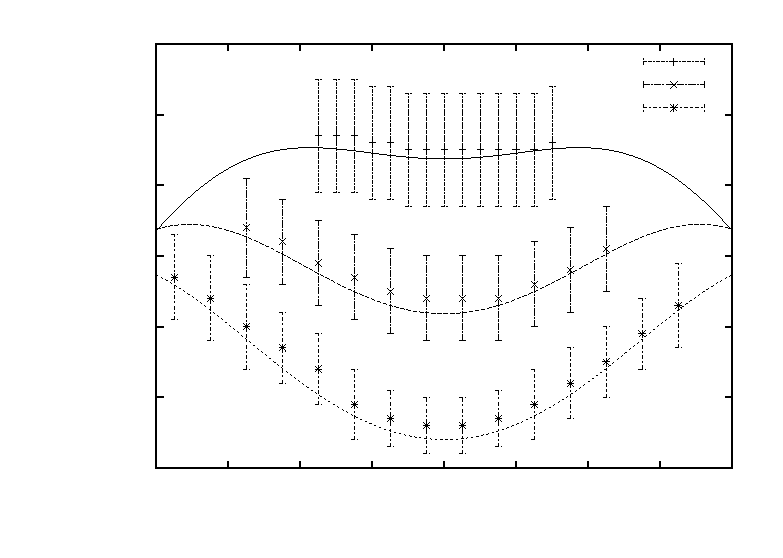
\includegraphics{g1}}%
    \gplfronttext
  \end{picture}%
\endgroup

\caption{Graf závislosti velikosti intenzity magnetického pole na poloze pro různě vzdálenosti cívek při souhlasném směru proudu.}
\label{g1}
\end{figure}

\begin{figure}
% GNUPLOT: LaTeX picture with Postscript
\begingroup
  \makeatletter
  \providecommand\color[2][]{%
    \GenericError{(gnuplot) \space\space\space\@spaces}{%
      Package color not loaded in conjunction with
      terminal option `colourtext'%
    }{See the gnuplot documentation for explanation.%
    }{Either use 'blacktext' in gnuplot or load the package
      color.sty in LaTeX.}%
    \renewcommand\color[2][]{}%
  }%
  \providecommand\includegraphics[2][]{%
    \GenericError{(gnuplot) \space\space\space\@spaces}{%
      Package graphicx or graphics not loaded%
    }{See the gnuplot documentation for explanation.%
    }{The gnuplot epslatex terminal needs graphicx.sty or graphics.sty.}%
    \renewcommand\includegraphics[2][]{}%
  }%
  \providecommand\rotatebox[2]{#2}%
  \@ifundefined{ifGPcolor}{%
    \newif\ifGPcolor
    \GPcolorfalse
  }{}%
  \@ifundefined{ifGPblacktext}{%
    \newif\ifGPblacktext
    \GPblacktexttrue
  }{}%
  % define a \g@addto@macro without @ in the name:
  \let\gplgaddtomacro\g@addto@macro
  % define empty templates for all commands taking text:
  \gdef\gplbacktext{}%
  \gdef\gplfronttext{}%
  \makeatother
  \ifGPblacktext
    % no textcolor at all
    \def\colorrgb#1{}%
    \def\colorgray#1{}%
  \else
    % gray or color?
    \ifGPcolor
      \def\colorrgb#1{\color[rgb]{#1}}%
      \def\colorgray#1{\color[gray]{#1}}%
      \expandafter\def\csname LTw\endcsname{\color{white}}%
      \expandafter\def\csname LTb\endcsname{\color{black}}%
      \expandafter\def\csname LTa\endcsname{\color{black}}%
      \expandafter\def\csname LT0\endcsname{\color[rgb]{1,0,0}}%
      \expandafter\def\csname LT1\endcsname{\color[rgb]{0,1,0}}%
      \expandafter\def\csname LT2\endcsname{\color[rgb]{0,0,1}}%
      \expandafter\def\csname LT3\endcsname{\color[rgb]{1,0,1}}%
      \expandafter\def\csname LT4\endcsname{\color[rgb]{0,1,1}}%
      \expandafter\def\csname LT5\endcsname{\color[rgb]{1,1,0}}%
      \expandafter\def\csname LT6\endcsname{\color[rgb]{0,0,0}}%
      \expandafter\def\csname LT7\endcsname{\color[rgb]{1,0.3,0}}%
      \expandafter\def\csname LT8\endcsname{\color[rgb]{0.5,0.5,0.5}}%
    \else
      % gray
      \def\colorrgb#1{\color{black}}%
      \def\colorgray#1{\color[gray]{#1}}%
      \expandafter\def\csname LTw\endcsname{\color{white}}%
      \expandafter\def\csname LTb\endcsname{\color{black}}%
      \expandafter\def\csname LTa\endcsname{\color{black}}%
      \expandafter\def\csname LT0\endcsname{\color{black}}%
      \expandafter\def\csname LT1\endcsname{\color{black}}%
      \expandafter\def\csname LT2\endcsname{\color{black}}%
      \expandafter\def\csname LT3\endcsname{\color{black}}%
      \expandafter\def\csname LT4\endcsname{\color{black}}%
      \expandafter\def\csname LT5\endcsname{\color{black}}%
      \expandafter\def\csname LT6\endcsname{\color{black}}%
      \expandafter\def\csname LT7\endcsname{\color{black}}%
      \expandafter\def\csname LT8\endcsname{\color{black}}%
    \fi
  \fi
  \setlength{\unitlength}{0.0500bp}%
  \begin{picture}(7200.00,5040.00)%
    \gplgaddtomacro\gplbacktext{%
      \csname LTb\endcsname%
      \put(1078,704){\makebox(0,0)[r]{\strut{} 0}}%
      \put(1078,1286){\makebox(0,0)[r]{\strut{} 100}}%
      \put(1078,1867){\makebox(0,0)[r]{\strut{} 200}}%
      \put(1078,2449){\makebox(0,0)[r]{\strut{} 300}}%
      \put(1078,3030){\makebox(0,0)[r]{\strut{} 400}}%
      \put(1078,3612){\makebox(0,0)[r]{\strut{} 500}}%
      \put(1078,4193){\makebox(0,0)[r]{\strut{} 600}}%
      \put(1078,4775){\makebox(0,0)[r]{\strut{} 700}}%
      \put(1210,484){\makebox(0,0){\strut{}-8}}%
      \put(1917,484){\makebox(0,0){\strut{}-6}}%
      \put(2625,484){\makebox(0,0){\strut{}-4}}%
      \put(3332,484){\makebox(0,0){\strut{}-2}}%
      \put(4040,484){\makebox(0,0){\strut{} 0}}%
      \put(4747,484){\makebox(0,0){\strut{} 2}}%
      \put(5454,484){\makebox(0,0){\strut{} 4}}%
      \put(6162,484){\makebox(0,0){\strut{} 6}}%
      \put(6869,484){\makebox(0,0){\strut{} 8}}%
      \put(308,2739){\rotatebox{-270}{\makebox(0,0){\strut{}$H$/Am$^{-1}$}}}%
      \put(4039,154){\makebox(0,0){\strut{}$x$/cm}}%
    }%
    \gplgaddtomacro\gplfronttext{%
      \csname LTb\endcsname%
      \put(5882,4602){\makebox(0,0)[r]{\strut{}12 cm}}%
      \csname LTb\endcsname%
      \put(5882,4382){\makebox(0,0)[r]{\strut{}16 cm}}%
      \csname LTb\endcsname%
      \put(5882,4162){\makebox(0,0)[r]{\strut{}20 cm}}%
    }%
    \gplbacktext
    \put(0,0){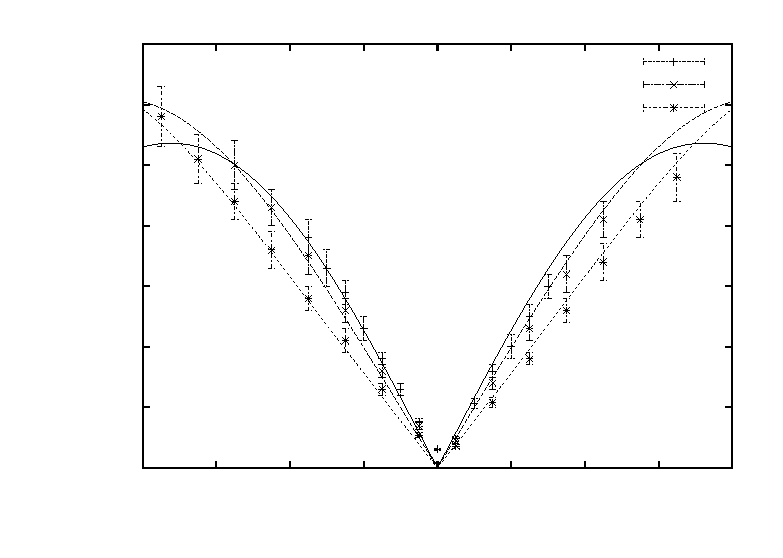
\includegraphics{g2}}%
    \gplfronttext
  \end{picture}%
\endgroup

\caption{Graf závislosti velikosti intenzity magnetického pole na poloze pro různě vzdálenosti cívek při nesouhlasném směru proudu.}
\label{g2}
\end{figure}

\subsection{Úkol 2}
Následně jsem měřil velikost intenzity magnetického pole uprostřed cívek pro jejich různé vzdálenosti. To jsem opět vypočítal dle vztahu \ref{H3} 
z naměřeného indukovaného napětí. Výsledné hodnoty jsou v tabulce \ref{d} a na obrázku \ref{g3} opět se zanesenou teoretickou závislostí.

\begin{table}
$$
\begin{array}{|c|c|}
\hline
d/\mbox{cm}& H/\mbox{Am}^{-1} \\ \hline
7& 1200\pm100 \\ \hline
8&  1180\pm90 \\ \hline
9&  1120\pm90 \\ \hline
10& 1060\pm80   \\ \hline
11& 1010\pm80 \\ \hline
12& 950\pm80    \\ \hline
13& 890\pm70 \\ \hline
14& 840\pm70    \\ \hline
15& 790\pm60 \\ \hline
16& 740\pm60    \\ \hline
17& 690\pm50 \\ \hline
18& 640\pm50    \\ \hline
19& 600\pm50 \\ \hline
20& 560\pm40    \\ \hline
\end{array}
$$
\caption{Tabulka závislosti velikosti intenzity magnetického pole uprostřed souosých cívek v závislosti na jejich vzdálenosti.}
\label{d}
\end{table}

\begin{figure}
% GNUPLOT: LaTeX picture with Postscript
\begingroup
  \makeatletter
  \providecommand\color[2][]{%
    \GenericError{(gnuplot) \space\space\space\@spaces}{%
      Package color not loaded in conjunction with
      terminal option `colourtext'%
    }{See the gnuplot documentation for explanation.%
    }{Either use 'blacktext' in gnuplot or load the package
      color.sty in LaTeX.}%
    \renewcommand\color[2][]{}%
  }%
  \providecommand\includegraphics[2][]{%
    \GenericError{(gnuplot) \space\space\space\@spaces}{%
      Package graphicx or graphics not loaded%
    }{See the gnuplot documentation for explanation.%
    }{The gnuplot epslatex terminal needs graphicx.sty or graphics.sty.}%
    \renewcommand\includegraphics[2][]{}%
  }%
  \providecommand\rotatebox[2]{#2}%
  \@ifundefined{ifGPcolor}{%
    \newif\ifGPcolor
    \GPcolorfalse
  }{}%
  \@ifundefined{ifGPblacktext}{%
    \newif\ifGPblacktext
    \GPblacktexttrue
  }{}%
  % define a \g@addto@macro without @ in the name:
  \let\gplgaddtomacro\g@addto@macro
  % define empty templates for all commands taking text:
  \gdef\gplbacktext{}%
  \gdef\gplfronttext{}%
  \makeatother
  \ifGPblacktext
    % no textcolor at all
    \def\colorrgb#1{}%
    \def\colorgray#1{}%
  \else
    % gray or color?
    \ifGPcolor
      \def\colorrgb#1{\color[rgb]{#1}}%
      \def\colorgray#1{\color[gray]{#1}}%
      \expandafter\def\csname LTw\endcsname{\color{white}}%
      \expandafter\def\csname LTb\endcsname{\color{black}}%
      \expandafter\def\csname LTa\endcsname{\color{black}}%
      \expandafter\def\csname LT0\endcsname{\color[rgb]{1,0,0}}%
      \expandafter\def\csname LT1\endcsname{\color[rgb]{0,1,0}}%
      \expandafter\def\csname LT2\endcsname{\color[rgb]{0,0,1}}%
      \expandafter\def\csname LT3\endcsname{\color[rgb]{1,0,1}}%
      \expandafter\def\csname LT4\endcsname{\color[rgb]{0,1,1}}%
      \expandafter\def\csname LT5\endcsname{\color[rgb]{1,1,0}}%
      \expandafter\def\csname LT6\endcsname{\color[rgb]{0,0,0}}%
      \expandafter\def\csname LT7\endcsname{\color[rgb]{1,0.3,0}}%
      \expandafter\def\csname LT8\endcsname{\color[rgb]{0.5,0.5,0.5}}%
    \else
      % gray
      \def\colorrgb#1{\color{black}}%
      \def\colorgray#1{\color[gray]{#1}}%
      \expandafter\def\csname LTw\endcsname{\color{white}}%
      \expandafter\def\csname LTb\endcsname{\color{black}}%
      \expandafter\def\csname LTa\endcsname{\color{black}}%
      \expandafter\def\csname LT0\endcsname{\color{black}}%
      \expandafter\def\csname LT1\endcsname{\color{black}}%
      \expandafter\def\csname LT2\endcsname{\color{black}}%
      \expandafter\def\csname LT3\endcsname{\color{black}}%
      \expandafter\def\csname LT4\endcsname{\color{black}}%
      \expandafter\def\csname LT5\endcsname{\color{black}}%
      \expandafter\def\csname LT6\endcsname{\color{black}}%
      \expandafter\def\csname LT7\endcsname{\color{black}}%
      \expandafter\def\csname LT8\endcsname{\color{black}}%
    \fi
  \fi
  \setlength{\unitlength}{0.0500bp}%
  \begin{picture}(7200.00,5040.00)%
    \gplgaddtomacro\gplbacktext{%
      \csname LTb\endcsname%
      \put(1210,704){\makebox(0,0)[r]{\strut{} 0}}%
      \put(1210,1382){\makebox(0,0)[r]{\strut{} 500}}%
      \put(1210,2061){\makebox(0,0)[r]{\strut{} 1000}}%
      \put(1210,2739){\makebox(0,0)[r]{\strut{} 1500}}%
      \put(1210,3418){\makebox(0,0)[r]{\strut{} 2000}}%
      \put(1210,4096){\makebox(0,0)[r]{\strut{} 2500}}%
      \put(1210,4775){\makebox(0,0)[r]{\strut{} 3000}}%
      \put(1342,484){\makebox(0,0){\strut{} 30}}%
      \put(1956,484){\makebox(0,0){\strut{} 40}}%
      \put(2570,484){\makebox(0,0){\strut{} 50}}%
      \put(3184,484){\makebox(0,0){\strut{} 60}}%
      \put(3798,484){\makebox(0,0){\strut{} 70}}%
      \put(4413,484){\makebox(0,0){\strut{} 80}}%
      \put(5027,484){\makebox(0,0){\strut{} 90}}%
      \put(5641,484){\makebox(0,0){\strut{} 100}}%
      \put(6255,484){\makebox(0,0){\strut{} 110}}%
      \put(6869,484){\makebox(0,0){\strut{} 120}}%
      \put(308,2739){\rotatebox{-270}{\makebox(0,0){\strut{}$f$/Hz}}}%
      \put(4105,154){\makebox(0,0){\strut{}$U_0$/V}}%
    }%
    \gplgaddtomacro\gplfronttext{%
    }%
    \gplbacktext
    \put(0,0){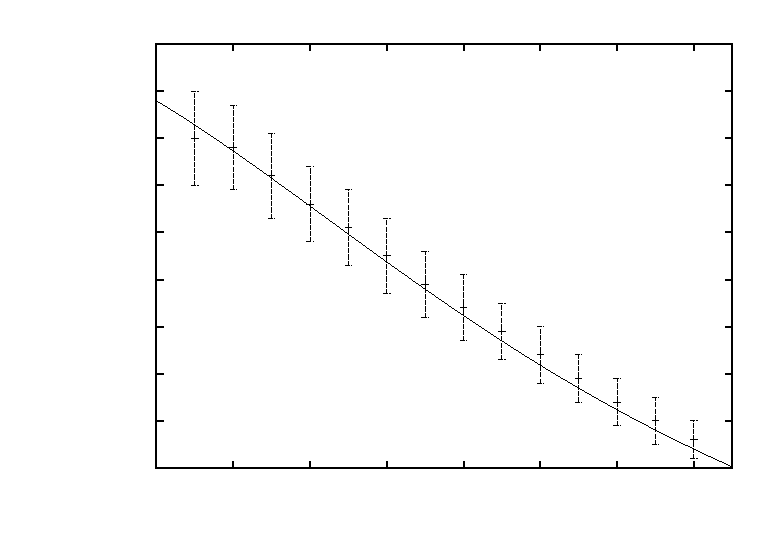
\includegraphics{g3}}%
    \gplfronttext
  \end{picture}%
\endgroup

\caption{Graf závislosti velikosti intenzity magnetického pole uprostřed cívek na jejich vzdálenosti.}
\label{g3}
\end{figure}

\subsection{Úkol 3}
Naměřil jsem indukované napětí pro různé body na ose při Helmholtzově poloze cívek. Dle \ref{H3} jsem vypočetl velikost magnetické indukce. 
Tyto hodnoty jsou v tabulce \ref{Helm}. Následně jsem je zanesl do grafu, kde jsem je proložil přímkou a zanesl do něj též teoretickou hodnotu. 
Výsledkem jest obrázek \ref{g4}. Dle programu gnuplot je střední hodnota velikosti intenzity rovna
\begin{eqnarray}
H=1045 \mbox{Am}^{-1}, 
\end{eqnarray}
což se od teoretické liší pouze o 1\%. Konstanta úměrnosti mezi intenzitou magnetického pole a napětím indukovaném na detekční cívce je dle vztahu (6) z \cite{text}
\begin{eqnarray}
k=(4900\pm400)\frac{\mbox{V}}{\mbox{mA}}
\label{k}
\end{eqnarray}

\begin{table}
$$
\begin{array}{|c|c|}
\hline
x/\mbox{cm}&    H/\mbox{Am}^{-1} \\ \hline
2.5&    1040\pm80   \\ \hline
3&  1050\pm 80  \\ \hline
3.5&    1050\pm80   \\ \hline
4&  1050\pm80   \\ \hline
4.5&    1050\pm80   \\ \hline
5&  1050\pm80   \\ \hline
5.5&    1050\pm80   \\ \hline
6&  1040\pm80   \\ \hline
6.5&    1040\pm80   \\ \hline
7&  1040\pm80   \\ \hline
7.5&    1040\pm80   \\ \hline
\end{array}
$$
\caption{Tabulka závislosti velikosti intenzity magnetického pole na poloze při Helmholtzově zapojení. }
\label{Helm}
\end{table}

\begin{figure}
% GNUPLOT: LaTeX picture with Postscript
\begingroup
  \makeatletter
  \providecommand\color[2][]{%
    \GenericError{(gnuplot) \space\space\space\@spaces}{%
      Package color not loaded in conjunction with
      terminal option `colourtext'%
    }{See the gnuplot documentation for explanation.%
    }{Either use 'blacktext' in gnuplot or load the package
      color.sty in LaTeX.}%
    \renewcommand\color[2][]{}%
  }%
  \providecommand\includegraphics[2][]{%
    \GenericError{(gnuplot) \space\space\space\@spaces}{%
      Package graphicx or graphics not loaded%
    }{See the gnuplot documentation for explanation.%
    }{The gnuplot epslatex terminal needs graphicx.sty or graphics.sty.}%
    \renewcommand\includegraphics[2][]{}%
  }%
  \providecommand\rotatebox[2]{#2}%
  \@ifundefined{ifGPcolor}{%
    \newif\ifGPcolor
    \GPcolorfalse
  }{}%
  \@ifundefined{ifGPblacktext}{%
    \newif\ifGPblacktext
    \GPblacktexttrue
  }{}%
  % define a \g@addto@macro without @ in the name:
  \let\gplgaddtomacro\g@addto@macro
  % define empty templates for all commands taking text:
  \gdef\gplbacktext{}%
  \gdef\gplfronttext{}%
  \makeatother
  \ifGPblacktext
    % no textcolor at all
    \def\colorrgb#1{}%
    \def\colorgray#1{}%
  \else
    % gray or color?
    \ifGPcolor
      \def\colorrgb#1{\color[rgb]{#1}}%
      \def\colorgray#1{\color[gray]{#1}}%
      \expandafter\def\csname LTw\endcsname{\color{white}}%
      \expandafter\def\csname LTb\endcsname{\color{black}}%
      \expandafter\def\csname LTa\endcsname{\color{black}}%
      \expandafter\def\csname LT0\endcsname{\color[rgb]{1,0,0}}%
      \expandafter\def\csname LT1\endcsname{\color[rgb]{0,1,0}}%
      \expandafter\def\csname LT2\endcsname{\color[rgb]{0,0,1}}%
      \expandafter\def\csname LT3\endcsname{\color[rgb]{1,0,1}}%
      \expandafter\def\csname LT4\endcsname{\color[rgb]{0,1,1}}%
      \expandafter\def\csname LT5\endcsname{\color[rgb]{1,1,0}}%
      \expandafter\def\csname LT6\endcsname{\color[rgb]{0,0,0}}%
      \expandafter\def\csname LT7\endcsname{\color[rgb]{1,0.3,0}}%
      \expandafter\def\csname LT8\endcsname{\color[rgb]{0.5,0.5,0.5}}%
    \else
      % gray
      \def\colorrgb#1{\color{black}}%
      \def\colorgray#1{\color[gray]{#1}}%
      \expandafter\def\csname LTw\endcsname{\color{white}}%
      \expandafter\def\csname LTb\endcsname{\color{black}}%
      \expandafter\def\csname LTa\endcsname{\color{black}}%
      \expandafter\def\csname LT0\endcsname{\color{black}}%
      \expandafter\def\csname LT1\endcsname{\color{black}}%
      \expandafter\def\csname LT2\endcsname{\color{black}}%
      \expandafter\def\csname LT3\endcsname{\color{black}}%
      \expandafter\def\csname LT4\endcsname{\color{black}}%
      \expandafter\def\csname LT5\endcsname{\color{black}}%
      \expandafter\def\csname LT6\endcsname{\color{black}}%
      \expandafter\def\csname LT7\endcsname{\color{black}}%
      \expandafter\def\csname LT8\endcsname{\color{black}}%
    \fi
  \fi
  \setlength{\unitlength}{0.0500bp}%
  \begin{picture}(7200.00,5040.00)%
    \gplgaddtomacro\gplbacktext{%
      \csname LTb\endcsname%
      \put(1210,704){\makebox(0,0)[r]{\strut{} 900}}%
      \put(1210,1383){\makebox(0,0)[r]{\strut{} 950}}%
      \put(1210,2061){\makebox(0,0)[r]{\strut{} 1000}}%
      \put(1210,2740){\makebox(0,0)[r]{\strut{} 1050}}%
      \put(1210,3418){\makebox(0,0)[r]{\strut{} 1100}}%
      \put(1210,4097){\makebox(0,0)[r]{\strut{} 1150}}%
      \put(1210,4775){\makebox(0,0)[r]{\strut{} 1200}}%
      \put(1342,484){\makebox(0,0){\strut{} 2}}%
      \put(2263,484){\makebox(0,0){\strut{} 3}}%
      \put(3184,484){\makebox(0,0){\strut{} 4}}%
      \put(4105,484){\makebox(0,0){\strut{} 5}}%
      \put(5027,484){\makebox(0,0){\strut{} 6}}%
      \put(5948,484){\makebox(0,0){\strut{} 7}}%
      \put(6869,484){\makebox(0,0){\strut{} 8}}%
      \put(308,2739){\rotatebox{-270}{\makebox(0,0){\strut{}$H$/Am$^{-1}$}}}%
      \put(4105,154){\makebox(0,0){\strut{}$x$/cm}}%
    }%
    \gplgaddtomacro\gplfronttext{%
      \csname LTb\endcsname%
      \put(5882,4602){\makebox(0,0)[r]{\strut{}teoretická}}%
      \csname LTb\endcsname%
      \put(5882,4382){\makebox(0,0)[r]{\strut{}fitovaná}}%
    }%
    \gplbacktext
    \put(0,0){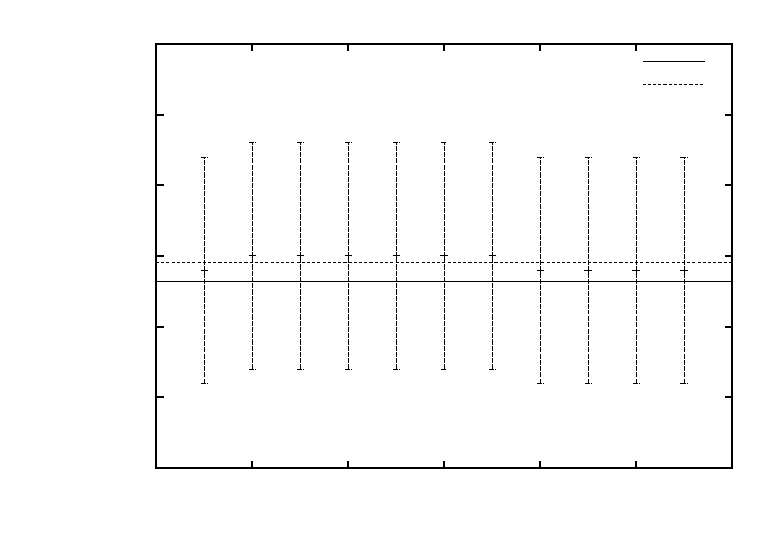
\includegraphics{g4}}%
    \gplfronttext
  \end{picture}%
\endgroup

\caption{Graf závislosti velikosti intenzity magnetického pole na poloze pro Helmholtzovo zapojení.}
\label{g4}
\end{figure}

\subsection{Úkol 4}
Nakonec jsem proměřoval velkosti intenzity magnetického pole uvnitř solenoidu. Počátek souřadného ssystěmu je přibližně na okraji cívky. 
Jeho parametry byly: $N=4204$, $l=400$ mm, $r_1=40$ mm, $r_2=70$ mm. Parametry detekční cívky byly $R=10.5$ mm a $N=370$. 
Indukci jsem opět vypočetl dle \ref{H3} z naměřeného napětí. Výsledky jsou v tabulce \ref{sol} a na obrázku \ref{g5} spolu 
s teoretickou křivkou dle předpisu \ref{TSol} dofitovanou pomocí programu gnuplot, který dopočetl její posunutí o 20.3 cm, protože tento vztah platí pro souřeadnice od středu solenoidu.

\begin{table}
$$
\begin{array}{|c|c||c|c|}
\hline
x/\mbox{cm}&    H/\mbox{Am}^{-1}&   x/\mbox{cm}&    H/\mbox{Am}^{-1} \\ \hline
0&   2300\pm    200&20&  5000\pm    400 \\ \hline
1&   2800\pm    200&22&  5000\pm    400 \\ \hline
2&   3300\pm    300&23&  5000\pm    400 \\ \hline
3&   3700\pm    300&24&  5000\pm    400 \\ \hline
4&   4000\pm    300&25&  5000\pm    400 \\ \hline
5&   4200\pm    300&26&  5000\pm    400 \\ \hline
6&   4400\pm    400&27&  4900\pm    400 \\ \hline
7&   4500\pm    400&28&  4900\pm    400 \\ \hline
8&   4600\pm    400&29&  4900\pm    400 \\ \hline
9&   4700\pm    400&30&  4800\pm    400 \\ \hline
10&  4800\pm    400&31&  4800\pm    400 \\ \hline
11&  4800\pm    400&32&  4700\pm    400 \\ \hline
12&  4900\pm    400&33&  4600\pm    400 \\ \hline
13&  4900\pm    400&34&  4500\pm    400 \\ \hline
14&  4900\pm    400&35&  4300\pm    300 \\ \hline
15&  4900\pm    400&36&  4000\pm    300 \\ \hline
16&  5000\pm    400&37&  3900\pm    300 \\ \hline
17&  5000\pm    400&38&  3400\pm    300 \\ \hline
18&  5000\pm    400&39&  2900\pm    200 \\ \hline
19&  5000\pm    400&& \\ \hline
\end{array}
$$
\caption{Tabulka velikosti intenzity magnetického pole uvnitř solenoidu v závislosti na poloze.}
\label{sol}
\end{table}
\begin{figure}
% GNUPLOT: LaTeX picture with Postscript
\begingroup
  \makeatletter
  \providecommand\color[2][]{%
    \GenericError{(gnuplot) \space\space\space\@spaces}{%
      Package color not loaded in conjunction with
      terminal option `colourtext'%
    }{See the gnuplot documentation for explanation.%
    }{Either use 'blacktext' in gnuplot or load the package
      color.sty in LaTeX.}%
    \renewcommand\color[2][]{}%
  }%
  \providecommand\includegraphics[2][]{%
    \GenericError{(gnuplot) \space\space\space\@spaces}{%
      Package graphicx or graphics not loaded%
    }{See the gnuplot documentation for explanation.%
    }{The gnuplot epslatex terminal needs graphicx.sty or graphics.sty.}%
    \renewcommand\includegraphics[2][]{}%
  }%
  \providecommand\rotatebox[2]{#2}%
  \@ifundefined{ifGPcolor}{%
    \newif\ifGPcolor
    \GPcolorfalse
  }{}%
  \@ifundefined{ifGPblacktext}{%
    \newif\ifGPblacktext
    \GPblacktexttrue
  }{}%
  % define a \g@addto@macro without @ in the name:
  \let\gplgaddtomacro\g@addto@macro
  % define empty templates for all commands taking text:
  \gdef\gplbacktext{}%
  \gdef\gplfronttext{}%
  \makeatother
  \ifGPblacktext
    % no textcolor at all
    \def\colorrgb#1{}%
    \def\colorgray#1{}%
  \else
    % gray or color?
    \ifGPcolor
      \def\colorrgb#1{\color[rgb]{#1}}%
      \def\colorgray#1{\color[gray]{#1}}%
      \expandafter\def\csname LTw\endcsname{\color{white}}%
      \expandafter\def\csname LTb\endcsname{\color{black}}%
      \expandafter\def\csname LTa\endcsname{\color{black}}%
      \expandafter\def\csname LT0\endcsname{\color[rgb]{1,0,0}}%
      \expandafter\def\csname LT1\endcsname{\color[rgb]{0,1,0}}%
      \expandafter\def\csname LT2\endcsname{\color[rgb]{0,0,1}}%
      \expandafter\def\csname LT3\endcsname{\color[rgb]{1,0,1}}%
      \expandafter\def\csname LT4\endcsname{\color[rgb]{0,1,1}}%
      \expandafter\def\csname LT5\endcsname{\color[rgb]{1,1,0}}%
      \expandafter\def\csname LT6\endcsname{\color[rgb]{0,0,0}}%
      \expandafter\def\csname LT7\endcsname{\color[rgb]{1,0.3,0}}%
      \expandafter\def\csname LT8\endcsname{\color[rgb]{0.5,0.5,0.5}}%
    \else
      % gray
      \def\colorrgb#1{\color{black}}%
      \def\colorgray#1{\color[gray]{#1}}%
      \expandafter\def\csname LTw\endcsname{\color{white}}%
      \expandafter\def\csname LTb\endcsname{\color{black}}%
      \expandafter\def\csname LTa\endcsname{\color{black}}%
      \expandafter\def\csname LT0\endcsname{\color{black}}%
      \expandafter\def\csname LT1\endcsname{\color{black}}%
      \expandafter\def\csname LT2\endcsname{\color{black}}%
      \expandafter\def\csname LT3\endcsname{\color{black}}%
      \expandafter\def\csname LT4\endcsname{\color{black}}%
      \expandafter\def\csname LT5\endcsname{\color{black}}%
      \expandafter\def\csname LT6\endcsname{\color{black}}%
      \expandafter\def\csname LT7\endcsname{\color{black}}%
      \expandafter\def\csname LT8\endcsname{\color{black}}%
    \fi
  \fi
  \setlength{\unitlength}{0.0500bp}%
  \begin{picture}(7200.00,5040.00)%
    \gplgaddtomacro\gplbacktext{%
      \csname LTb\endcsname%
      \put(1210,704){\makebox(0,0)[r]{\strut{} 1500}}%
      \put(1210,1213){\makebox(0,0)[r]{\strut{} 2000}}%
      \put(1210,1722){\makebox(0,0)[r]{\strut{} 2500}}%
      \put(1210,2231){\makebox(0,0)[r]{\strut{} 3000}}%
      \put(1210,2739){\makebox(0,0)[r]{\strut{} 3500}}%
      \put(1210,3248){\makebox(0,0)[r]{\strut{} 4000}}%
      \put(1210,3757){\makebox(0,0)[r]{\strut{} 4500}}%
      \put(1210,4266){\makebox(0,0)[r]{\strut{} 5000}}%
      \put(1210,4775){\makebox(0,0)[r]{\strut{} 5500}}%
      \put(1593,484){\makebox(0,0){\strut{} 0}}%
      \put(2221,484){\makebox(0,0){\strut{} 5}}%
      \put(2849,484){\makebox(0,0){\strut{} 10}}%
      \put(3477,484){\makebox(0,0){\strut{} 15}}%
      \put(4105,484){\makebox(0,0){\strut{} 20}}%
      \put(4734,484){\makebox(0,0){\strut{} 25}}%
      \put(5362,484){\makebox(0,0){\strut{} 30}}%
      \put(5990,484){\makebox(0,0){\strut{} 35}}%
      \put(6618,484){\makebox(0,0){\strut{} 40}}%
      \put(308,2739){\rotatebox{-270}{\makebox(0,0){\strut{}$H$/Am$^{-1}$}}}%
      \put(4105,154){\makebox(0,0){\strut{}$x$/cm}}%
    }%
    \gplgaddtomacro\gplfronttext{%
    }%
    \gplbacktext
    \put(0,0){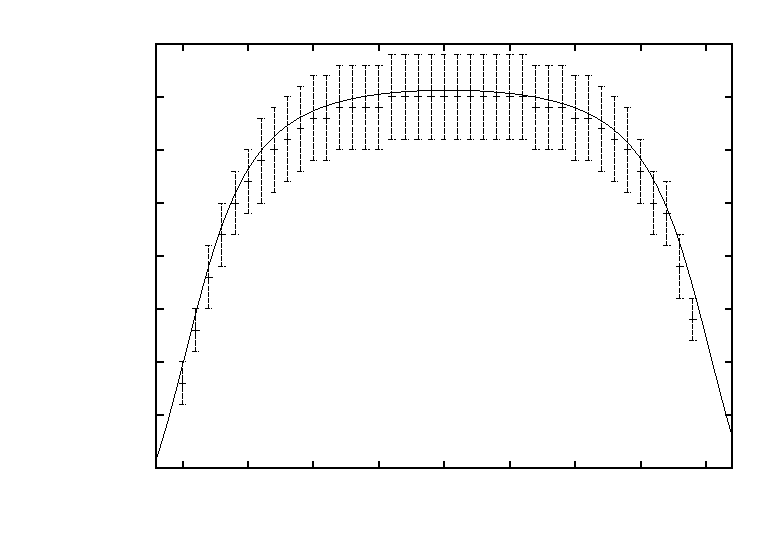
\includegraphics{g5}}%
    \gplfronttext
  \end{picture}%
\endgroup

\caption{Graf závislosti velikosti intenzity magnetického pole uvnitř solenoidu na poloze.}
\label{g5}
\end{figure}

\section{Diskuze}
Celková chyba měření se dosahuje přibližně 8 \%. To je způsobeno velkou nepřímou chybou z rovnice \ref{H3}. Tři veličiny v ní vystupující 
jsou zadané v \cite{text}, kde bohužel není zadána jejich chyba. Z toho důvodu jsem ji mohl pouze odhadnout, takže skutečná chyba je možná 
o něco menší. 

Naměřené hodnoty vesměs odpovídají těm teoretickým. Drobné odchylky jsou způsobeny pravděpodobně lehkou idealizací úlohy, kdy cívky nejsou 
nekonečně krátké, což se podle mě projevuje zejména u detekční cívky. V úloze 4 by také přesnosti napomohl lepší rozsah volmetr, protože jsem 
chybě odhadl velikost indukovaného napětí a proto byl rozsah zbytečně velký.

\section{Závěr}
\noindent
Změřil jsem průběh intenzity magnetického pole na ose souosých kruhových cívek
    \begin{enumerate}
    \item v zapojení se souhlasným směrem proudu. Výsledky jsou v tabulce \ref{souhlas} a na obrázku~\ref{g1}.
    \item v zapojení s nesouhlasným směrem proudu. Výsledky jsou v tabulce \ref{nesouhlas} a na obrázku~\ref{g2}.
    \end{enumerate}

Změřil jsem intenzitu magnetického pole uprostřed osy souosých cívek pro jejich různé vzdálenosti. Výsledky jsou v tabulce \ref{d} a na obrázku \ref{g3}.

Přesvědčil jsem se o homogenitě magnetického pole při Helmholtzově poloze cívek (tabulka \ref{Helm} a obrázek \ref{g4}) a stanovil experimentální hodnotu konstanty úměrnosti pod vztahem \ref{k}.

Proměřil jsem průběh intenzity magnetického pole uvnitř solenoidu. Výsledky jsou v tabulce \ref{sol} a na obrázku \ref{g5}. 

Do všech grafů jsem zanesl i jejich teoretické průběhy.

\begin{thebibliography}{5}
	\bibitem{text} \textbf{Studijní text na praktikum II} \\http://physics.mff.cuni.cz/vyuka/zfp/txt\_223.pdf (19. 10. 2011)
    \bibitem{chyba} \emph{J. Englich}: \textbf{Zpracování výsldků fyzikálních měření} \\ LS 1999/2000
\end{thebibliography}

\end{document}
